%!TeX root=../emmatop.tex
\chapter[Chapter \thechapter]{}
\lettrine[lines=4,lraise=0.3]{M}{r} Knightley might quarrel with her, but Emma could not quarrel with herself. He was so much displeased, that it was longer than usual before he came to Hartfield again; and when they did meet, his grave looks shewed that she was not forgiven. She was sorry, but could not repent. On the contrary, her plans and proceedings were more and more justified and endeared to her by the general appearances of the next few days.

The Picture, elegantly framed, came safely to hand soon after Mr Elton's return, and being hung over the mantelpiece of the common sitting-room, he got up to look at it, and sighed out his half sentences of admiration just as he ought; and as for Harriet's feelings, they were visibly forming themselves into as strong and steady an attachment as her youth and sort of mind admitted. Emma was soon perfectly satisfied of Mr Martin's being no otherwise remembered, than as he furnished a contrast with Mr Elton, of the utmost advantage to the latter.

Her views of improving her little friend's mind, by a great deal of useful reading and conversation, had never yet led to more than a few first chapters, and the intention of going on to-morrow. It was much easier to chat than to study; much pleasanter to let her imagination range and work at Harriet's fortune, than to be labouring to enlarge her comprehension or exercise it on sober facts; and the only literary pursuit which engaged Harriet at present, the only mental provision she was making for the evening of life, was the collecting and transcribing all the riddles of every sort that she could meet with, into a thin quarto of hot-pressed paper, made up by her friend, and ornamented with ciphers and trophies.

In this age of literature, such collections on a very grand scale are not uncommon. Miss Nash, head-teacher at Mrs Goddard's, had written out at least three hundred; and Harriet, who had taken the first hint of it from her, hoped, with Miss Woodhouse's help, to get a great many more. Emma assisted with her invention, memory and taste; and as Harriet wrote a very pretty hand, it was likely to be an arrangement of the first order, in form as well as quantity.

Mr Woodhouse was almost as much interested in the business as the girls, and tried very often to recollect something worth their putting in. »So many clever riddles as there used to be when he was young—he wondered he could not remember them! but he hoped he should in time.« And it always ended in »Kitty, a fair but frozen maid.«

His good friend Perry, too, whom he had spoken to on the subject, did not at present recollect any thing of the riddle kind; but he had desired Perry to be upon the watch, and as he went about so much, something, he thought, might come from that quarter.

It was by no means his daughter's wish that the intellects of Highbury in general should be put under requisition. Mr Elton was the only one whose assistance she asked. He was invited to contribute any really good enigmas, charades, or conundrums that he might recollect; and she had the pleasure of seeing him most intently at work with his recollections; and at the same time, as she could perceive, most earnestly careful that nothing ungallant, nothing that did not breathe a compliment to the sex should pass his lips. They owed to him their two or three politest puzzles; and the joy and exultation with which at last he recalled, and rather sentimentally recited, that well-known charade,

\begin{verse}
\begin{altverse}
My first doth affliction denote,\\
    Which my second is destin'd to feel\\
And my whole is the best antidote\\
    That affliction to soften and heal.—\\
\end{altverse}
\end{verse}

made her quite sorry to acknowledge that they had transcribed it some pages ago already.

»Why will not you write one yourself for us, Mr Elton?« said she; »that is the only security for its freshness; and nothing could be easier to you.«

»Oh no! he had never written, hardly ever, any thing of the kind in his life. The stupidest fellow! He was afraid not even Miss Woodhouse«—he stopt a moment—»or Miss Smith could inspire him.«

The very next day however produced some proof of inspiration. He called for a few moments, just to leave a piece of paper on the table containing, as he said, a charade, which a friend of his had addressed to a young lady, the object of his admiration, but which, from his manner, Emma was immediately convinced must be his own.

»I do not offer it for Miss Smith's collection,« said he. »Being my friend's, I have no right to expose it in any degree to the public eye, but perhaps you may not dislike looking at it.«

The speech was more to Emma than to Harriet, which Emma could understand. There was deep consciousness about him, and he found it easier to meet her eye than her friend's. He was gone the next moment:—after another moment's pause,

»Take it,« said Emma, smiling, and pushing the paper towards Harriet—»it is for you. Take your own.«

But Harriet was in a tremor, and could not touch it; and Emma, never loth to be first, was obliged to examine it herself.

\begin{quotation}
To Miss——

\textsc{charade.}

\begin{verse}
\begin{altverse}
My first displays the wealth and pomp of kings,\\
    Lords of the earth! their luxury and ease.\\
Another view of man, my second brings,\\
    Behold him there, the monarch of the seas!\\

But ah! united, what reverse we have!\\
    Man's boasted power and freedom, all are flown;\\
Lord of the earth and sea, he bends a slave,\\
    And woman, lovely woman, reigns alone.\\

    Thy ready wit the word will soon supply,\\
    May its approval beam in that soft eye!\\
\end{altverse}
\end{verse}
\end{quotation}

She cast her eye over it, pondered, caught the meaning, read it through again to be quite certain, and quite mistress of the lines, and then passing it to Harriet, sat happily smiling, and saying to herself, while Harriet was puzzling over the paper in all the confusion of hope and dulness, »Very well, Mr Elton, very well indeed. I have read worse charades. \textit{Courtship}—a very good hint. I give you credit for it. This is feeling your way. This is saying very plainly—»Pray, Miss Smith, give me leave to pay my addresses to you. Approve my charade and my intentions in the same glance.«

\begin{quote}
May its approval beam in that soft eye!
\end{quote}


Harriet exactly. Soft is the very word for her eye—of all epithets, the justest that could be given.

\begin{quote}
Thy ready wit the word will soon supply.
\end{quote}


Humph—Harriet's ready wit! All the better. A man must be very much in love, indeed, to describe her so. Ah! Mr Knightley, I wish you had the benefit of this; I think this would convince you. For once in your life you would be obliged to own yourself mistaken. An excellent charade indeed! and very much to the purpose. Things must come to a crisis soon now.«

She was obliged to break off from these very pleasant observations, which were otherwise of a sort to run into great length, by the eagerness of Harriet's wondering questions.

»What can it be, Miss Woodhouse?—what can it be? I have not an idea—I cannot guess it in the least. What can it possibly be? Do try to find it out, Miss Woodhouse. Do help me. I never saw any thing so hard. Is it kingdom? I wonder who the friend was—and who could be the young lady. Do you think it is a good one? Can it be woman?

\begin{quote}
And woman, lovely woman, reigns alone.
\end{quote}

Can it be Neptune?

\begin{quote}
Behold him there, the monarch of the seas!
\end{quote}


Or a trident? or a mermaid? or a shark? Oh, no! shark is only one syllable. It must be very clever, or he would not have brought it. Oh! Miss Woodhouse, do you think we shall ever find it out?«

»Mermaids and sharks! Nonsense! My dear Harriet, what are you thinking of? Where would be the use of his bringing us a charade made by a friend upon a mermaid or a shark? Give me the paper and listen.«

»For Miss ———,«read Miss Smith.

\begin{verse}
\begin{altverse}
My first displays the wealth and pomp of kings,\\
    Lords of the earth! their luxury and ease.
\end{altverse}
\end{verse}

That is \textit{court}.

\begin{verse}
\begin{altverse}
Another view of man, my second brings;\\
    Behold him there, the monarch of the seas!
	\end{altverse}
\end{verse}

That is \textit{ship};—plain as it can be.—Now for the cream.

\begin{verse}
\begin{altverse}
But ah! united, (\textit{courtship}, you know,) what reverse we have!\\
    Man's boasted power and freedom, all are flown.\\
Lord of the earth and sea, he bends a slave,\\
    And woman, lovely woman, reigns alone.\\
	
	\end{altverse}
\end{verse}

»A very proper compliment!—and then follows the application, which I think, my dear Harriet, you cannot find much difficulty in comprehending. Read it in comfort to yourself. There can be no doubt of its being written for you and to you.«

Harriet could not long resist so delightful a persuasion. She read the concluding lines, and was all flutter and happiness. She could not speak. But she was not wanted to speak. It was enough for her to feel. Emma spoke for her.

»There is so pointed, and so particular a meaning in this compliment,« said she, »that I cannot have a doubt as to Mr Elton's intentions. You are his object—and you will soon receive the completest proof of it. I thought it must be so. I thought I could not be so deceived; but now, it is clear; the state of his mind is as clear and decided, as my wishes on the subject have been ever since I knew you. Yes, Harriet, just so long have I been wanting the very circumstance to happen that has happened. I could never tell whether an attachment between you and Mr Elton were most desirable or most natural. Its probability and its eligibility have really so equalled each other! I am very happy. I congratulate you, my dear Harriet, with all my heart. This is an attachment which a woman may well feel pride in creating. This is a connexion which offers nothing but good. It will give you every thing that you want—consideration, independence, a proper home—it will fix you in the centre of all your real friends, close to Hartfield and to me, and confirm our intimacy for ever. This, Harriet, is an alliance which can never raise a blush in either of us.«

»Dear Miss Woodhouse!«—and »Dear Miss Woodhouse,« was all that Harriet, with many tender embraces could articulate at first; but when they did arrive at something more like conversation, it was sufficiently clear to her friend that she saw, felt, anticipated, and remembered just as she ought. Mr Elton's superiority had very ample acknowledgment.

»Whatever you say is always right,« cried Harriet, »and therefore I suppose, and believe, and hope it must be so; but otherwise I could not have imagined it. It is so much beyond any thing I deserve. Mr Elton, who might marry any body! There cannot be two opinions about \textit{him}. He is so very superior. Only think of those sweet verses—»To Miss ———.« Dear me, how clever!—Could it really be meant for me?«

»I cannot make a question, or listen to a question about that. It is a certainty. Receive it on my judgment. It is a sort of prologue to the play, a motto to the chapter; and will be soon followed by matter-of-fact prose.«

»It is a sort of thing which nobody could have expected. I am sure, a month ago, I had no more idea myself!—The strangest things do take place!«

»When Miss Smiths and Mr Eltons get acquainted—they do indeed—and really it is strange; it is out of the common course that what is so evidently, so palpably desirable—what courts the pre-arrangement of other people, should so immediately shape itself into the proper form. You and Mr Elton are by situation called together; you belong to one another by every circumstance of your respective homes. Your marrying will be equal to the match at Randalls. There does seem to be a something in the air of Hartfield which gives love exactly the right direction, and sends it into the very channel where it ought to flow.

\begin{quote}
The course of true love never did run smooth—
\end{quote}

\begin{letter}
	\enlargethispage{\baselineskip}
\end{letter}

A Hartfield edition of Shakespeare would have a long note on that passage.«

»That Mr Elton should really be in love with me,—me, of all people, who did not know him, to speak to him, at Michaelmas! And he, the very handsomest man that ever was, and a man that every body looks up to, quite like Mr Knightley! His company so sought after, that every body says he need not eat a single meal by himself if he does not chuse it; that he has more invitations than there are days in the week. And so excellent in the Church! Miss Nash has put down all the texts he has ever preached from since he came to Highbury. Dear me! When I look back to the first time I saw him! How little did I think!—The two Abbots and I ran into the front room and peeped through the blind when we heard he was going by, and Miss Nash came and scolded us away, and staid to look through herself; however, she called me back presently, and let me look too, which was very good-natured. And how beautiful we thought he looked! He was arm-in-arm with Mr Cole.«

»This is an alliance which, whoever—whatever your friends may be, must be agreeable to them, provided at least they have common sense; and we are not to be addressing our conduct to fools. If they are anxious to see you \textit{happily} married, here is a man whose amiable character gives every assurance of it;—if they wish to have you settled in the same country and circle which they have chosen to place you in, here it will be accomplished; and if their only object is that you should, in the common phrase, be \textit{well} married, here is the comfortable fortune, the respectable establishment, the rise in the world which must satisfy them.«

»Yes, very true. How nicely you talk; I love to hear you. You understand every thing. You and Mr Elton are one as clever as the other. This charade!—If I had studied a twelvemonth, I could never have made any thing like it.«

»I thought he meant to try his skill, by his manner of declining it yesterday.«

»I do think it is, without exception, the best charade I ever read.«

»I never read one more to the purpose, certainly.«

»It is as long again as almost all we have had before.«

»I do not consider its length as particularly in its favour. Such things in general cannot be too short.«

Harriet was too intent on the lines to hear. The most satisfactory comparisons were rising in her mind.

»It is one thing,« said she, presently—her cheeks in a glow—»to have very good sense in a common way, like every body else, and if there is any thing to say, to sit down and write a letter, and say just what you must, in a short way; and another, to write verses and charades like this.«

Emma could not have desired a more spirited rejection of Mr Martin's prose.

»Such sweet lines!« continued Harriet—»these two last!—But how shall I ever be able to return the paper, or say I have found it out?—Oh! Miss Woodhouse, what can we do about that?«

»Leave it to me. You do nothing. He will be here this evening, I dare say, and then I will give it him back, and some nonsense or other will pass between us, and you shall not be committed.—Your soft eyes shall chuse their own time for beaming. Trust to me.«

»Oh! Miss Woodhouse, what a pity that I must not write this beautiful charade into my book! I am sure I have not got one half so good.«

»Leave out the two last lines, and there is no reason why you should not write it into your book.«

»Oh! but those two lines are«—

—»The best of all. Granted;—for private enjoyment; and for private enjoyment keep them. They are not at all the less written you know, because you divide them. The couplet does not cease to be, nor does its meaning change. But take it away, and all \textit{appropriation} ceases, and a very pretty gallant charade remains, fit for any collection. Depend upon it, he would not like to have his charade slighted, much better than his passion. A poet in love must be encouraged in both capacities, or neither. Give me the book, I will write it down, and then there can be no possible reflection on you.«

Harriet submitted, though her mind could hardly separate the parts, so as to feel quite sure that her friend were not writing down a declaration of love. It seemed too precious an offering for any degree of publicity.

»I shall never let that book go out of my own hands,« said she.

»Very well,« replied Emma; »a most natural feeling; and the longer it lasts, the better I shall be pleased. But here is my father coming: you will not object to my reading the charade to him. It will be giving him so much pleasure! He loves any thing of the sort, and especially any thing that pays woman a compliment. He has the tenderest spirit of gallantry towards us all!—You must let me read it to him.«

Harriet looked grave.

»My dear Harriet, you must not refine too much upon this charade.—You will betray your feelings improperly, if you are too conscious and too quick, and appear to affix more meaning, or even quite all the meaning which may be affixed to it. Do not be overpowered by such a little tribute of admiration. If he had been anxious for secrecy, he would not have left the paper while I was by; but he rather pushed it towards me than towards you. Do not let us be too solemn on the business. He has encouragement enough to proceed, without our sighing out our souls over this charade.«

»Oh! no—I hope I shall not be ridiculous about it. Do as you please.«

Mr Woodhouse came in, and very soon led to the subject again, by the recurrence of his very frequent inquiry of »Well, my dears, how does your book go on?—Have you got any thing fresh?«

»Yes, papa; we have something to read you, something quite fresh. A piece of paper was found on the table this morning—(dropt, we suppose, by a fairy)—containing a very pretty charade, and we have just copied it in.«

She read it to him, just as he liked to have any thing read, slowly and distinctly, and two or three times over, with explanations of every part as she proceeded—and he was very much pleased, and, as she had foreseen, especially struck with the complimentary conclusion.

»Aye, that's very just, indeed, that's very properly said. Very true. »Woman, lovely woman.« It is such a pretty charade, my dear, that I can easily guess what fairy brought it.—Nobody could have written so prettily, but you, Emma.«

Emma only nodded, and smiled.—After a little thinking, and a very tender sigh, he added,

»Ah! it is no difficulty to see who you take after! Your dear mother was so clever at all those things! If I had but her memory! But I can remember nothing;—not even that particular riddle which you have heard me mention; I can only recollect the first stanza; and there are several.

\begin{letter}
	\clearpage 
\end{letter}

\begin{samepage}
\begin{verse}
Kitty, a fair but frozen maid,\\
    Kindled a flame I yet deplore,\\
The hood-wink'd boy I called to aid,\\
Though of his near approach afraid,\\
    So fatal to my suit before.\\
	\end{verse}
\end{samepage}

And that is all that I can recollect of it—but it is very clever all the way through. But I think, my dear, you said you had got it.«

»Yes, papa, it is written out in our second page. We copied it from the \textit{Elegant Extracts}. It was Garrick's, you know.«

»Aye, very true.—I wish I could recollect more of it.

\begin{quote}
Kitty, a fair but frozen maid.
\end{quote}

The name makes me think of poor Isabella; for she was very near being christened Catherine after her grandmama. I hope we shall have her here next week. Have you thought, my dear, where you shall put her—and what room there will be for the children?«

»Oh! yes—she will have her own room, of course; the room she always has;—and there is the nursery for the children,—just as usual, you know. Why should there be any change?«

»I do not know, my dear—but it is so long since she was here!—not since last Easter, and then only for a few days.—Mr John Knightley's being a lawyer is very inconvenient.—Poor Isabella!—she is sadly taken away from us all!—and how sorry she will be when she comes, not to see Miss Taylor here!«

»She will not be surprized, papa, at least.«

»I do not know, my dear. I am sure I was very much surprized when I first heard she was going to be married.«

»We must ask Mr and Mrs Weston to dine with us, while Isabella is here.«

»Yes, my dear, if there is time.—But—(in a very depressed tone)—she is coming for only one week. There will not be time for any thing.«

»It is unfortunate that they cannot stay longer—but it seems a case of necessity. Mr John Knightley must be in town again on the 28th, and we ought to be thankful, papa, that we are to have the whole of the time they can give to the country, that two or three days are not to be taken out for the Abbey. Mr Knightley promises to give up his claim this Christmas—though you know it is longer since they were with him, than with us.«

»It would be very hard, indeed, my dear, if poor Isabella were to be anywhere but at Hartfield.«

Mr Woodhouse could never allow for Mr Knightley's claims on his brother, or any body's claims on Isabella, except his own. He sat musing a little while, and then said,

»But I do not see why poor Isabella should be obliged to go back so soon, though he does. I think, Emma, I shall try and persuade her to stay longer with us. She and the children might stay very well.«

»Ah! papa—that is what you never have been able to accomplish, and I do not think you ever will. Isabella cannot bear to stay behind her husband.«

This was too true for contradiction. Unwelcome as it was, Mr Woodhouse could only give a submissive sigh; and as Emma saw his spirits affected by the idea of his daughter's attachment to her husband, she immediately led to such a branch of the subject as must raise them.

»Harriet must give us as much of her company as she can while my brother and sister are here. I am sure she will be pleased with the children. We are very proud of the children, are not we, papa? I wonder which she will think the handsomest, Henry or John?«

»Aye, I wonder which she will. Poor little dears, how glad they will be to come. They are very fond of being at Hartfield, Harriet.«

»I dare say they are, sir. I am sure I do not know who is not.«

»Henry is a fine boy, but John is very like his mama. Henry is the eldest, he was named after me, not after his father. John, the second, is named after his father. Some people are surprized, I believe, that the eldest was not, but Isabella would have him called Henry, which I thought very pretty of her. And he is a very clever boy, indeed. They are all remarkably clever; and they have so many pretty ways. They will come and stand by my chair, and say, »Grandpapa, can you give me a bit of string?« and once Henry asked me for a knife, but I told him knives were only made for grandpapas. I think their father is too rough with them very often.«

»He appears rough to you,« said Emma, »because you are so very gentle yourself; but if you could compare him with other papas, you would not think him rough. He wishes his boys to be active and hardy; and if they misbehave, can give them a sharp word now and then; but he is an affectionate father—certainly Mr John Knightley is an affectionate father. The children are all fond of him.«

\begin{figure}[tbph]
\centering
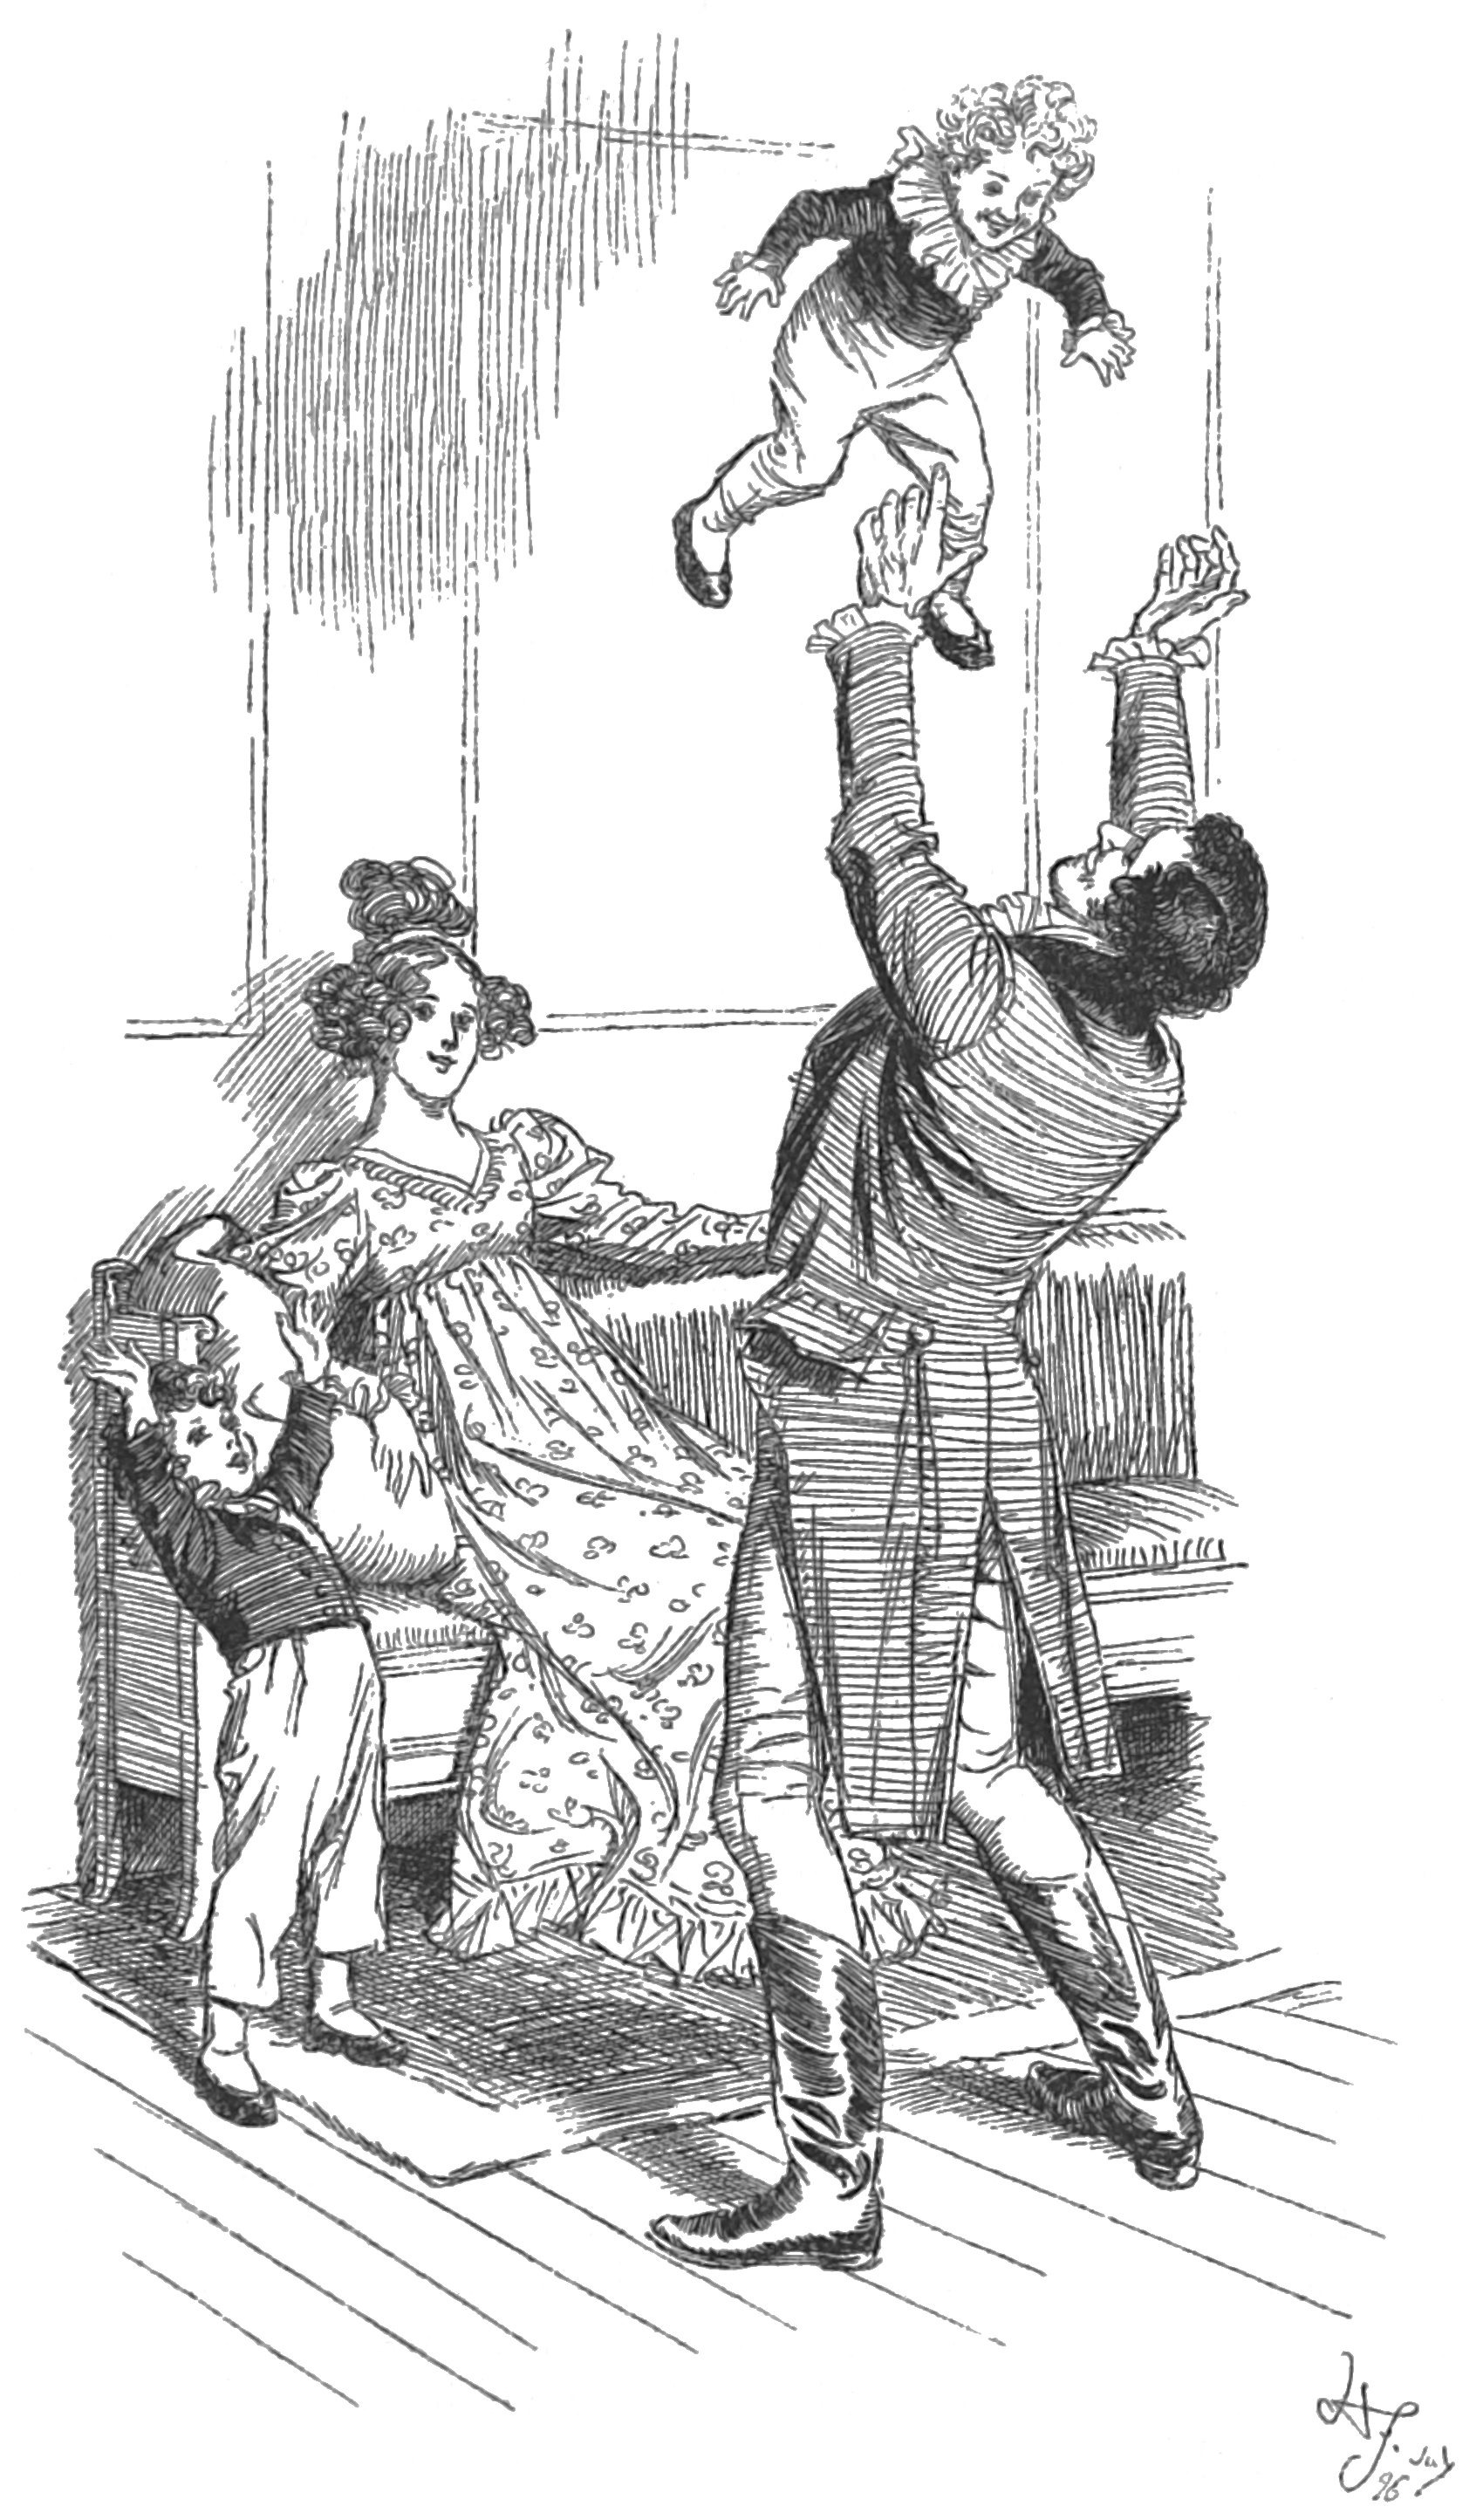
\includegraphics[width=.8\linewidth]{9ceiling}
\caption{Tosses them up to the ceiling}
\end{figure}

»And then their uncle comes in, and tosses them up to the ceiling in a very frightful way!«

»But they like it, papa; there is nothing they like so much. It is such enjoyment to them, that if their uncle did not lay down the rule of their taking turns, whichever began would never give way to the other.«

»Well, I cannot understand it.«

»That is the case with us all, papa. One half of the world cannot understand the pleasures of the other.«

Later in the morning, and just as the girls were going to separate in preparation for the regular four o'clock dinner, the hero of this inimitable charade walked in again. Harriet turned away; but Emma could receive him with the usual smile, and her quick eye soon discerned in his the consciousness of having made a push—of having thrown a die; and she imagined he was come to see how it might turn up. His ostensible reason, however, was to ask whether Mr Woodhouse's party could be made up in the evening without him, or whether he should be in the smallest degree necessary at Hartfield. If he were, every thing else must give way; but otherwise his friend Cole had been saying so much about his dining with him—had made such a point of it, that he had promised him conditionally to come.

Emma thanked him, but could not allow of his disappointing his friend on their account; her father was sure of his rubber. He re-urged—she re-declined; and he seemed then about to make his bow, when taking the paper from the table, she returned it—

»Oh! here is the charade you were so obliging as to leave with us; thank you for the sight of it. We admired it so much, that I have ventured to write it into Miss Smith's collection. Your friend will not take it amiss I hope. Of course I have not transcribed beyond the first eight lines.«

Mr Elton certainly did not very well know what to say. He looked rather doubtingly—rather confused; said something about »honour,«—glanced at Emma and at Harriet, and then seeing the book open on the table, took it up, and examined it very attentively. With the view of passing off an awkward moment, Emma smilingly said,

»You must make my apologies to your friend; but so good a charade must not be confined to one or two. He may be sure of every woman's approbation while he writes with such gallantry.«

»I have no hesitation in saying,« replied Mr Elton, though hesitating a good deal while he spoke; »I have no hesitation in saying—at least if my friend feels at all as \textit{I} do—I have not the smallest doubt that, could he see his little effusion honoured as \textit{I} see it, (looking at the book again, and replacing it on the table), he would consider it as the proudest moment of his life.«

After this speech he was gone as soon as possible. Emma could not think it too soon; for with all his good and agreeable qualities, there was a sort of parade in his speeches which was very apt to incline her to laugh. She ran away to indulge the inclination, leaving the tender and the sublime of pleasure to Harriet's share.